\documentclass[11pt,a4paper,notitlepage]{article}
\usepackage[utf8]{inputenc}
\usepackage[T1]{fontenc}
\usepackage{graphicx}
\usepackage{enumerate}
\usepackage{xcolor}
\definecolor{bg}{rgb}{0.95,0.95,0.95}
\usepackage{ulem}
\usepackage{listings}
\usepackage{vhistory}
\usepackage[parfill]{parskip}

\lstdefinestyle{BashInputStyle}{
  language=bash,
  basicstyle=\small\sffamily,
  commentstyle=\color{black},    
  numberstyle=\tiny\color{black}, 
  keywordstyle=\color{black},       
  extendedchars=true,              
  numbers=none,
  numbersep=3pt,
  frame=tb,
  columns=fullflexible,
  backgroundcolor=\color{yellow!20},
  linewidth=\linewidth,
  breaklines=true,
  breakatwhitespace=false,           
  showspaces=false,
  keepspaces=true,                 
  captionpos=b,                    
  showspaces=false,                
  showstringspaces=false,          
  showtabs=false,                  
  tabsize=2,                       
  aboveskip=\bigskipamount, 
  belowskip=\bigskipamount,
}

\author{Ananya Muddukrishna}
\date{ananya@kth.se}
\title{Annotated Task Graph (ATG)}

\begin{document}
\maketitle

% Start of the revision history table
\begin{versionhistory}
\vhEntry{1.0}{2014-06-19}{ananya} {Created}
\vhEntry{1.1}{2014-07-01}{ananya} {Improved ATG generation text}
\vhEntry{1.2}{2014-07-02}{ananya} {Simplified ATG generation text}
\end{versionhistory}

\section{Introduction}
The Annotated task Graph (ATG) refers to information obtained by the instruction-level profiling feature of the MIR runtime system library.
Instruction-level profiling is performed using a custom Pin call-graph profiling tool.

The ATG is available in two forms - a raw form and a visual form.

\section{Getting the ATG}
\label{sec:getting-atg}
Let us obtain the ATG for the fib program in MIR\_ROOT/test/fib.
The fib program takes two arguments. The first is the number n and the second is the depth cutoff for recursive task creation.

We first have to compile the fib program without aggressive optimizations and disable inlining so that outline functions representing tasks are visible to Pin call-graph profiler. 
Look at the SConstruct file in MIR\_ROOT/test/fib and build output to understand which arguments are supplied to the compiler to get the profiling-specialized executable called fib-prof. 
Build output pertaining to fib-prof are show below.

\begin{lstlisting}[style=BashInputStyle]
$ cd $MIR_ROOT/test/fib

$ scons 
scons: Reading SConscript files ...
scons: done reading SConscript files.
scons: Building targets ...
scons: building associated VariantDir targets: debug-build opt-build prof-build verbose-build
...
gcc -o prof-build/fib.o -c -std=c99 -Wall -Werror -Wno-unused-function -Wno-unused-variable -Wno-unused-but-set-variable -Wno-maybe-uninitialized -fopenmp -DLINUX -I/home/ananya/mir-dev/src -I/home/ananya/mir-dev/test/common -O1 -DNDEBUG -fno-inline-functions -fno-inline-functions-called-once -fno-optimize-sibling-calls -fno-omit-frame-pointer -g fib.c
...
gcc -o fib-prof prof-build/fib.o -L/home/ananya/mir-dev/src -lpthread -lm -lmir-opt
...
scons: done building targets.
\end{lstlisting}

We next identify outline functions and functions called within tasks of the fib program. 
To do so, we use a simple script - profiler\_params.py - which searches for known outline function name patterns within the object files of the program fib-prof. 
The script also lists all function symbols within the object files which we treat as potentially callable functions and filter those which are certianly called by tasks defined in the program. 
Inspecting program source files is a quick way to identify certainly called functions. 
By looking at fib program sources, we can exclude main and get\_usecs from the called functions list.
If in doubt or when sources are not available, use the entire callable function list.
Identifying function called by tasks is necessary because the instruction count of these functions are added to the calling task's instruction count.

\begin{lstlisting}[style=BashInputStyle]
$ cd $MIR_ROOT/test/fib

$ echo "Examining executable for names of outline and callable functions ..."
$ $MIR_ROOT/scripts/task-graph/profiler_params.py prof-build/*.o
Using "._omp_fn.|ol_" as outline function name pattern
Processing file: prof-build/fib.o
OUTLINE_FUNCTIONS=ol_fib_0,ol_fib_1,ol_fib_2
CALLABLE_FUNCTIONS=fib_seq,fib,get_usecs,main
\end{lstlisting}

Now we invoke the Pin call-graph profiler - mir\_outline\_function\_profiler.so - with appropriate arguments to profile fib-prof and obtain instruction-level information for tasks.
The profiler accepts outline function names under the argument -s and names of function which are called within tasks under the argument -c. 
The -o argument is used as suffix to file names produced during profiling.
The $--$ argument indicates the profiled program and its arguments, which in our case is fib-prof with inputs n=10 and cutoff=4.
Use the -h argument for help information about the profiler.
We additionally instruct MIR to provide fork-join task graph information using MIR\_CONF="-w=1 -g -p" which is mandatory and constant for building the ATG.
The MIR\_CONF argument -w=1 enables single-threaded execution, -g enables fork-join task graph building and -p enables hand-shaking between the MIR runtime system and the Pin call-graph profiler.
Use the -h argument for help information about MIR\_CONF.

\begin{lstlisting}[style=BashInputStyle]
$ LD_LIBRARY_PATH=$LD_LIBRARY_PATH:$PIN_ROOT/intel64/runtime \
    MIR_CONF="-w=1 -g -p" \
    $PIN_ROOT/intel64/bin/pinbin \
    -t ${MIR_ROOT}/scripts/task-graph/obj-intel64/mir_outline_function_profiler.so \
    -o fib_test \
    -s ol_fib_0,ol_fib_1,ol_fib_2 \
    -c fib,fib_seq \
    -- ./fib-prof 10 4

$ mv mir-task-graph fib_test-fork_join_task_graph
\end{lstlisting}

Now, we can get some basic task-based information by processing the fork-join task graph produced by MIR.
\begin{lstlisting}[style=BashInputStyle]
$ echo "Summarizing fork-join task graph ..."
$ Rscript ${MIR_ROOT}/scripts/task-graph/mir-fork-join-graph-info.R fib_test-fork_join_task_graph 
\end{lstlisting}

We can also plot the fork-join task graph. 
\begin{lstlisting}[style=BashInputStyle]
$ echo "Plotting fork-join task graph ..."
$ Rscript ${MIR_ROOT}/scripts/task-graph/mir-fork-join-graph-plot.R fib_test-fork_join_task_graph color
\end{lstlisting}

Now, we combine the instruction-level profile produced by the Pin call-graph profiler with the fork-join task graph information produced by MIR. We call this process as annotating the fork-join task graph with instruction-level information. The annotation process produces the raw format of the ATG.

\begin{lstlisting}[style=BashInputStyle]
$ echo "Annotating fork-join task graph ..."
$ Rscript ${MIR_ROOT}/scripts/task-graph/mir-annotate-graph.R fib_test-fork_join_task_graph fib_test-call_graph fib_test
\end{lstlisting}

We can plot the raw ATG format to produce the visual form of the ATG.
\begin{lstlisting}[style=BashInputStyle]
$ echo "Plotting annotated task graph ..."
$ Rscript ${MIR_ROOT}/scripts/task-graph/mir-annotated-graph-plot.R fib_test-annotated_task_graph color
\end{lstlisting}

Let us list the files produced by running the above commands. See Table~\ref{tab:atg-files} for a description of files produced.
\begin{lstlisting}[style=BashInputStyle]
$ echo "Listing ATG files ..."
$ ls fib_test*
\end{lstlisting}

\begin{table}[!htb]
\begin{tabular}{|p{5.5cm}|p{7cm}|}
\hline
\textbf{File name} & \textbf{Description} \\ \hline
fib\_test-call\_graph & Instruction-level information of tasks \\ \hline
fib\_test-mem\_map & Memory map of program execution  \\ \hline
fib\_test-fork\_join\_task\_graph & Parent-child task relationship and tgpid information \\ \hline
fib\_test-annotated\_task\_graph & Raw format of the ATG combining instruction-level and parent-child information \\ \hline
fib\_test-annotated\_task\_graph.adjm & Adjacent matrix representation of the visual format of ATG \\ \hline
fib\_test-annotated\_task\_graph.dot & Dot representation of the visual format of ATG \\ \hline
fib\_test-annotated\_task\_graph.edgelist & Edgelist representation of the visual format of ATG \\ \hline
fib\_test-annotated\_task\_graph.graphml & GraphML representation of the visual format of ATG \\ \hline
fib\_test-annotated\_task\_graph.info & Summary information about visual format of the ATG. Includes work, span and critical path from Cilk theory. \\ \hline
fib\_test-fork\_join\_task\_graph.adjm & Adjacent matrix representation of the visual format of ATG without instruction-level information \\ \hline
fib\_test-fork\_join\_task\_graph.dot & Dot representation of the visual format of ATG without instruction-level information \\ \hline
fib\_test-fork\_join\_task\_graph.edgelist & Edgelist representation of the visual format of ATG without instruction-level information \\ \hline
fib\_test-fork\_join\_task\_graph.graphml & GraphML representation of the visual format of ATG without instruction-level information \\ \hline
fib\_test-fork\_join\_task\_graph.info & Summary information about visual format of ATG without instruction-level information. Includes number of tasks and join degree distribution. \\ \hline
\end{tabular}
\caption{ATG files}
\label{tab:atg-files}
\end{table}

\section{Raw format of the ATG}
The ATG raw format is a csv file.

\begin{lstlisting}[style=BashInputStyle]
$ head fib_test-annotated_task_graph
"task","parent","joins_at","tgpid","ins_count","stack_read","stack_write","mem_fp","ccr","clr","mem_read","mem_write","name"
1,0,0,"0.",59,11,15,5,12,15,4,1,"ol_fib_2"
2,1,0,"1.",60,10,15,5,12,15,4,1,"ol_fib_0"
3,1,0,"2.",60,10,15,5,12,15,4,1,"ol_fib_1"
4,3,0,"1.2.",60,10,15,5,12,15,4,1,"ol_fib_0"
5,3,0,"2.2.",60,10,15,5,12,15,4,1,"ol_fib_1"
6,5,0,"1.2.2.",60,10,15,5,12,15,4,1,"ol_fib_0"
7,5,0,"2.2.2.",60,10,15,5,12,15,4,1,"ol_fib_1"
8,7,0,"1.2.2.2.",68,15,15,5,14,17,4,1,"ol_fib_0"
9,7,0,"2.2.2.2.",47,10,10,5,9,12,4,1,"ol_fib_1"
\end{lstlisting}

Each line shows properties of an explicit task executed by the program.
The first line shows names of the properties. 
Properties are also called annotations.
See Table~\ref{tab:raw-format}.

\begin{table}[!htb]
\begin{tabular}{|p{2cm}|p{10cm}|}
\hline
\textbf{Field} & \textbf{Description} \\ \hline
task & Identifier of the task \\ \hline
parent & Identifier of the parent task of the task \\ \hline
joins\_at & Indicates at which call to taskwait in the parent the task synchronized. Example: 0 indicates the task synchronized with the first call to taskwait in the parent. Several children can synchronize at the same call.  \\ \hline
tgpid & Indicates the task graph position identifier. See details below.  \\ \hline
ins\_count & Indicates total number of instructions executed by the task. Profiling parameters indicate which instructions to count. Typically, instructions part of runtime system calls are excluded and calls to statically-linked functions are included.  \\ \hline
stack\_read & Indicates number of read accesses to the stack while executing instructions  \\ \hline
stack\_write & Indicates number of write accesses to the stack while executing instructions \\ \hline
ccr & Computation to Communication ratio. Indicates number of instructions executed per read or write access to memory  \\ \hline
clr & Computation to Load ratio. Indicates number of instructions executed per read access to memory  \\ \hline
mem\_read & Indicates number of read accesses to memory (excluding stack) while executing instructions  \\ \hline
mem\_write & Indicates number of write accesses to memory (excluding stack) while executing instructions  \\ \hline
name & Indicates name of the outline function of the task \\ \hline
\end{tabular}
\caption{Raw format fields}
\label{tab:raw-format}
\end{table}

\subsection{Property tgpid}
The tgpid uniquely identifies a task irrespective of single-thread or many-thread execution. 
The format of tgpid is A.B.C.....<implied 0>

\begin{itemize}
\item 0. Represents the first task created. This is a special meaning.
\item A. means Ath child of the first task
\item A.B. means Ath child of task B.
\item A.B.C. means Ath child of task B.C.
\end{itemize}

NOTE: The tgpid is an experimental feature, not fully tested and subject to change.

\section{Visual format of the ATG}
The visual format gives shape to the raw format of the ATG.
It describes task-based execution in an intuitive manner allowing the programmer to spot performance problems.
The visual format can be viewed using graph visualization tools such as dot, yEd and cytoscape.
See Figure~\ref{fig:yed-atg} for visualization of the ATG on yEd and Figure~\ref{fig:dot-atg} for visualization of the ATG on Dot.
Details of the visual format are subject of a scientific paper under review and will be made available soon.

\begin{lstlisting}[style=BashInputStyle]
$ echo "Visualizing annotated task graph ..."
$ dot -Tps fib_test-annotated_task_graph.dot >  fib_test-annotated_task_graph.dot.ps
$ yed fib_test-annotated_task_graph.graphml
\end{lstlisting}

\begin{figure}[!ht]
\centering
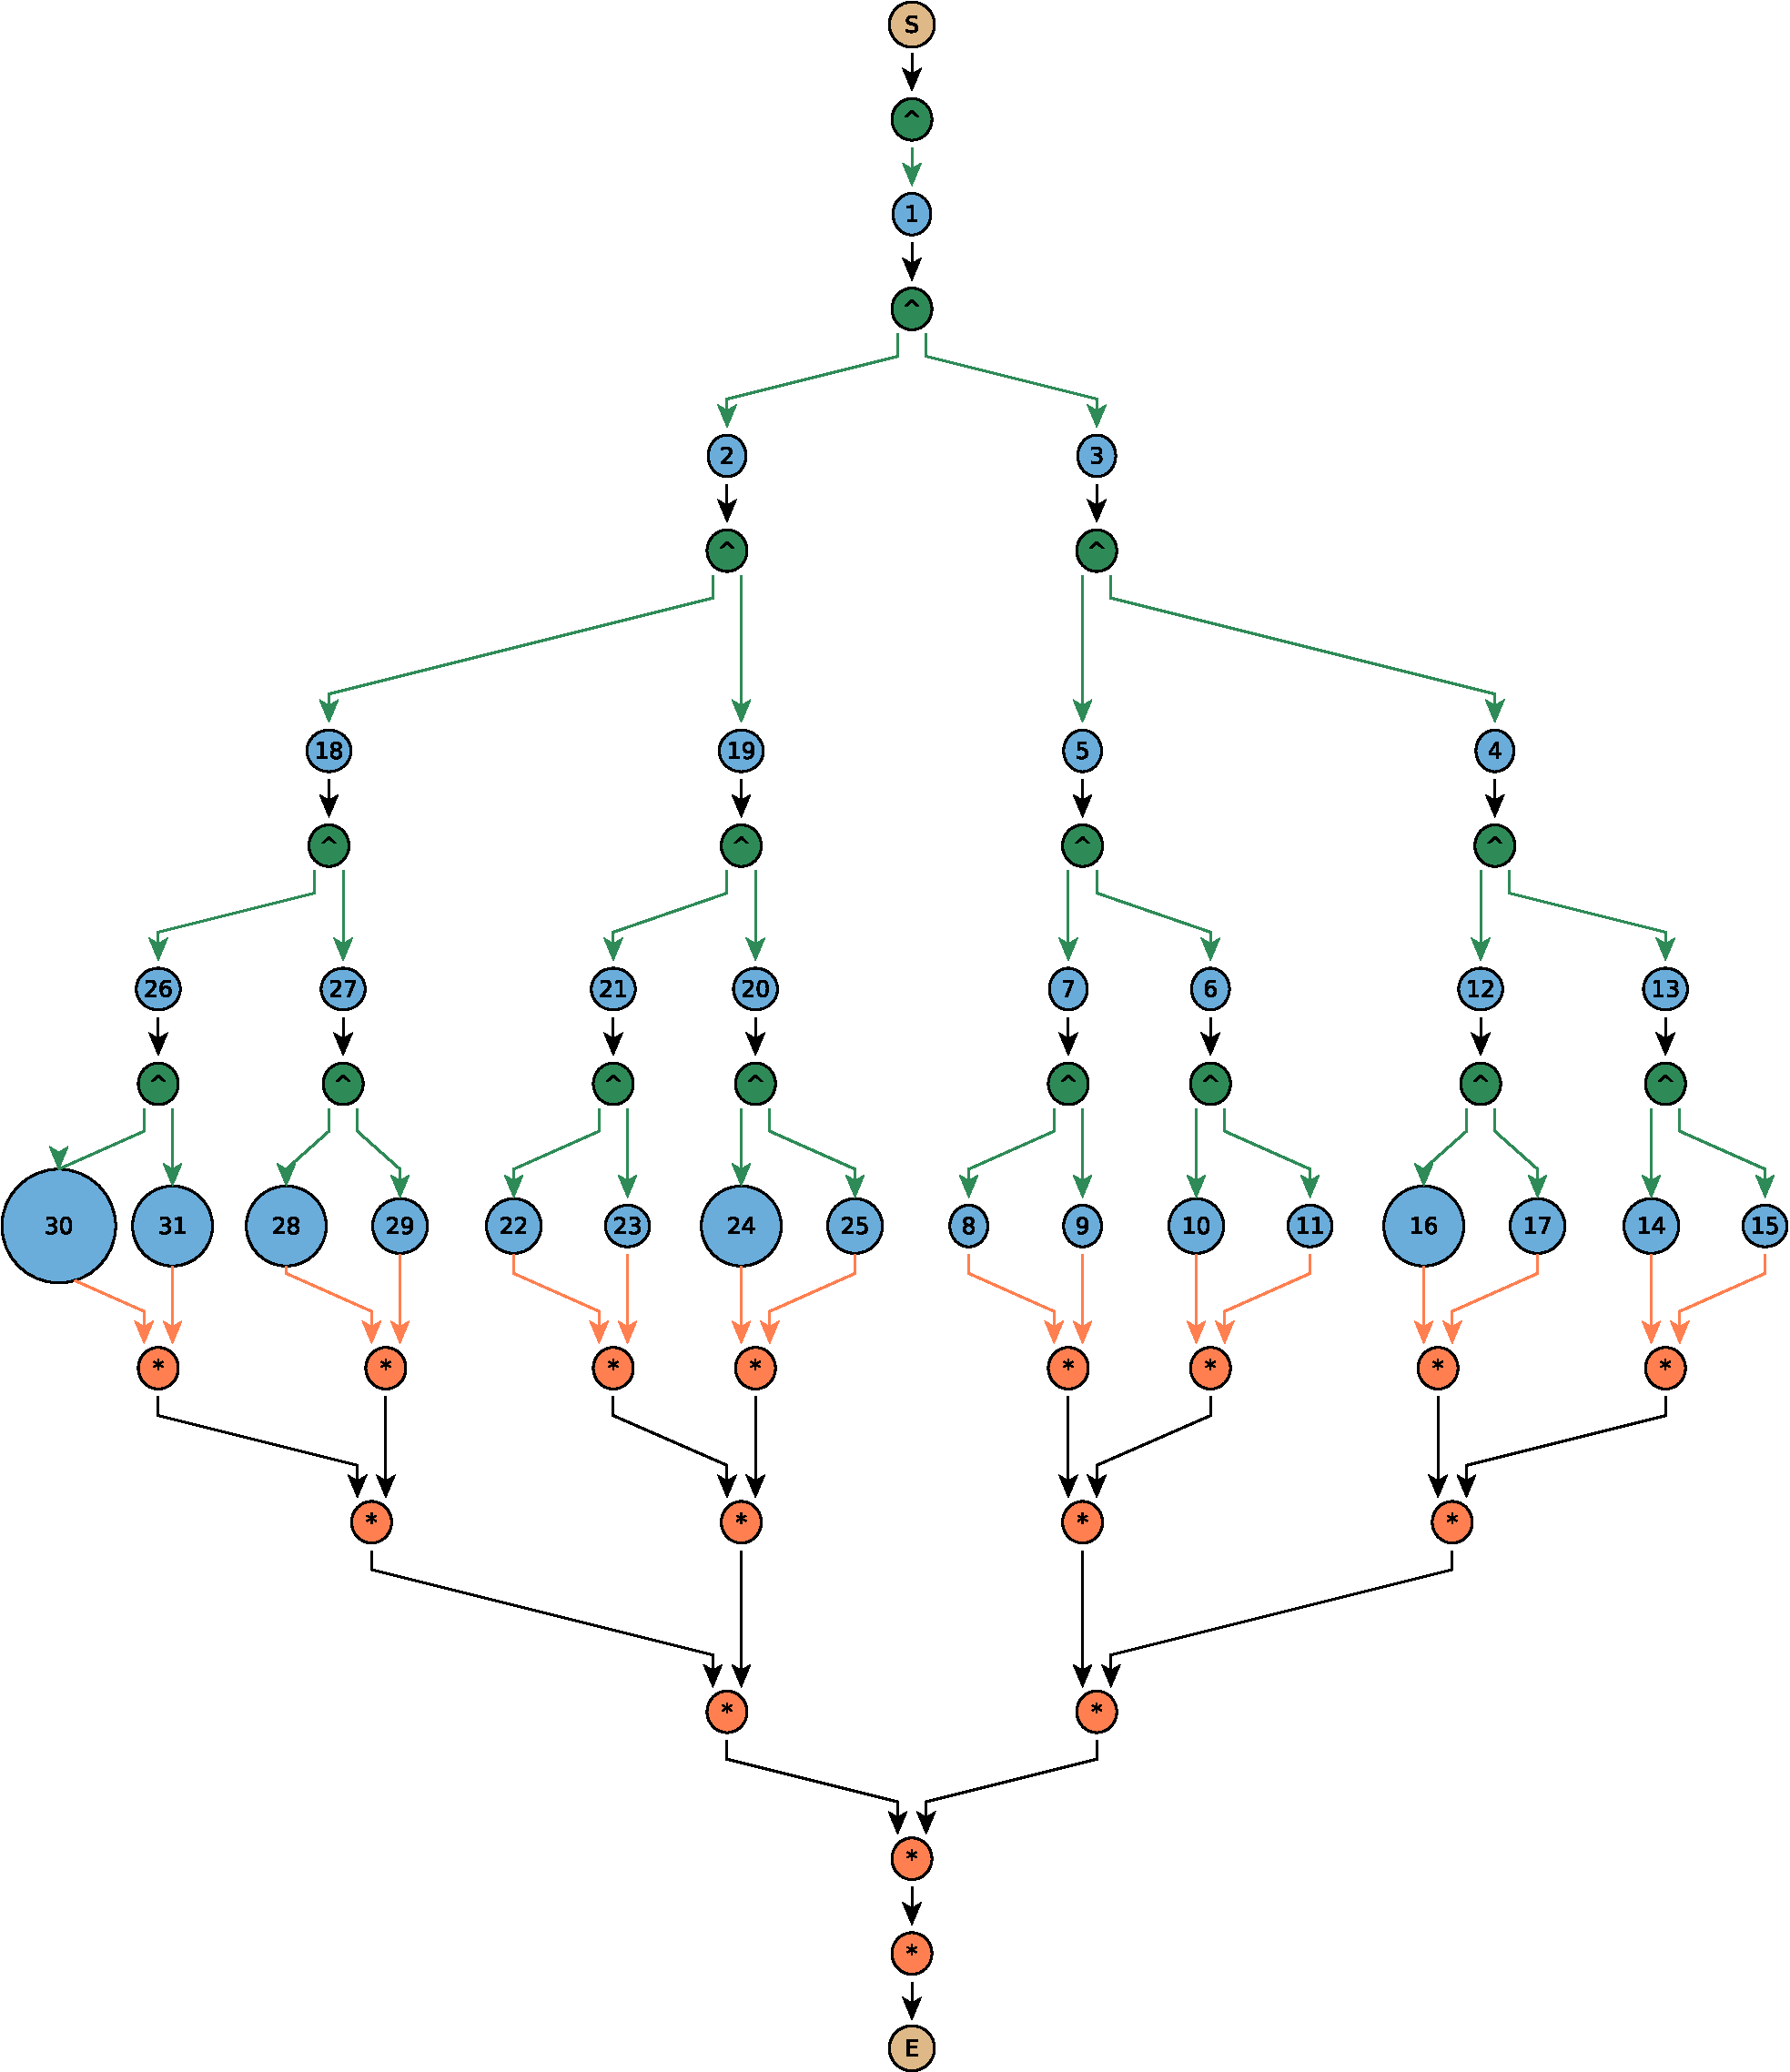
\includegraphics[width=\textwidth]{figures/fib_test-10_4-annotated_task_graph-yed.pdf}
\caption{fib\_test-annotated\_task\_graph.graphml viewed on yEd}
\label{fig:yed-atg}
\end{figure}

\begin{figure}[!ht]
\centering
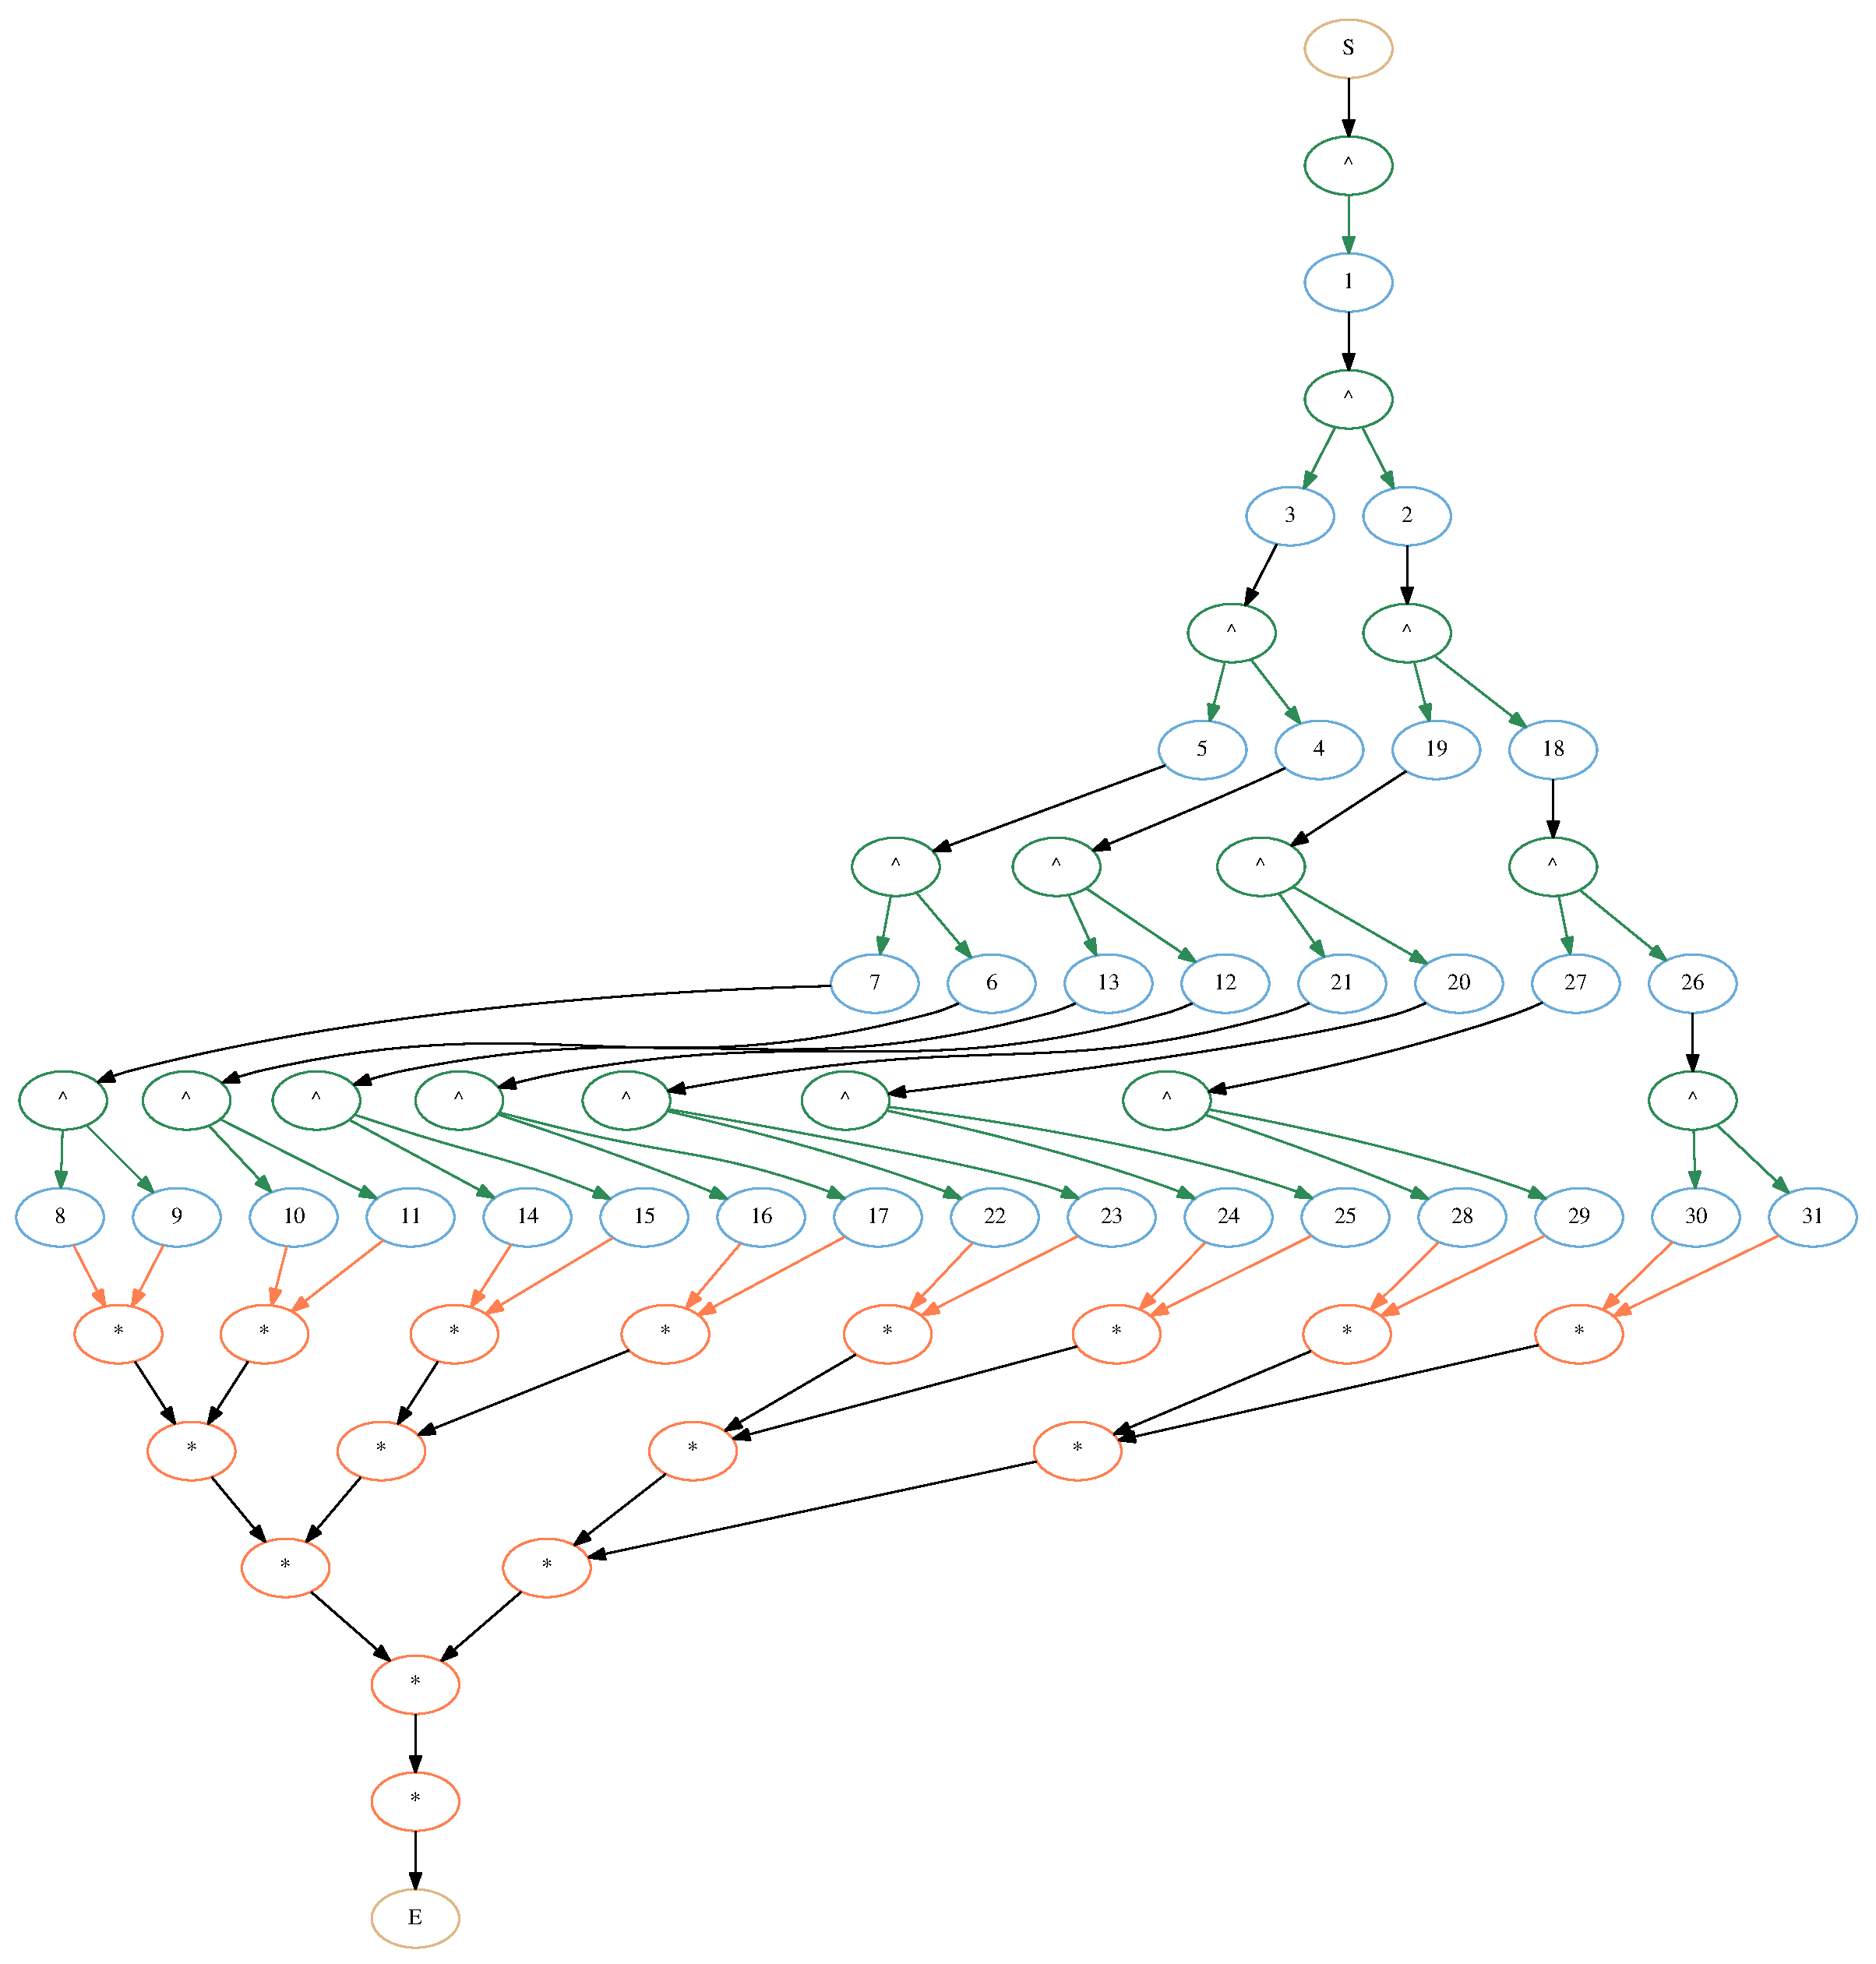
\includegraphics[width=\textwidth]{figures/fib_test-10_4-annotated_task_graph-dot.eps}
\caption{fib\_test-annotated\_task\_graph.dot visualized using Dot}
\label{fig:dot-atg}
\end{figure}

\end{document}
